\documentclass[12pt,a4paper]{scrartcl}
\usepackage[utf8]{inputenc}
\usepackage{amsmath}
\usepackage{amsfonts}
\usepackage{amssymb}
\usepackage{graphicx}


\usepackage[bottom = 1in, left = 0.5in, right = 0.5in, top = 1in]{geometry}

\usepackage[english]{babel}
\usepackage[autostyle]{csquotes}
% \usepackage{mathptmx}
\usepackage{bm}
\usepackage{caption}
\usepackage{float}
% Mark continued floats as a, b, ...
\renewcommand\theContinuedFloat{\roman{ContinuedFloat}}

\usepackage[labelfont=bf]{caption}

\usepackage[default, scale=0.95]{opensans} %% Alternatively
%% use the option 'defaultsans' instead of 'default' to replace the
%% sans serif font only.
\usepackage[T1]{fontenc}

\usepackage{titling}
\setlength{\droptitle}{-10em}   % This is your set screw

\addto\captionsenglish{\renewcommand{\figurename}{Supplementary Fig.}}
\addto\captionsenglish{\renewcommand{\tablename}{Supplementary Table}}

\usepackage{palatino}
\usepackage{textcomp}

\title{Supplementary materials}
\date{}

\begin{document}
\maketitle

\section*{Supplementary section 1}
\subsection*{Regions and ecosystems classification}

\begin{figure}[H]
	\centering
	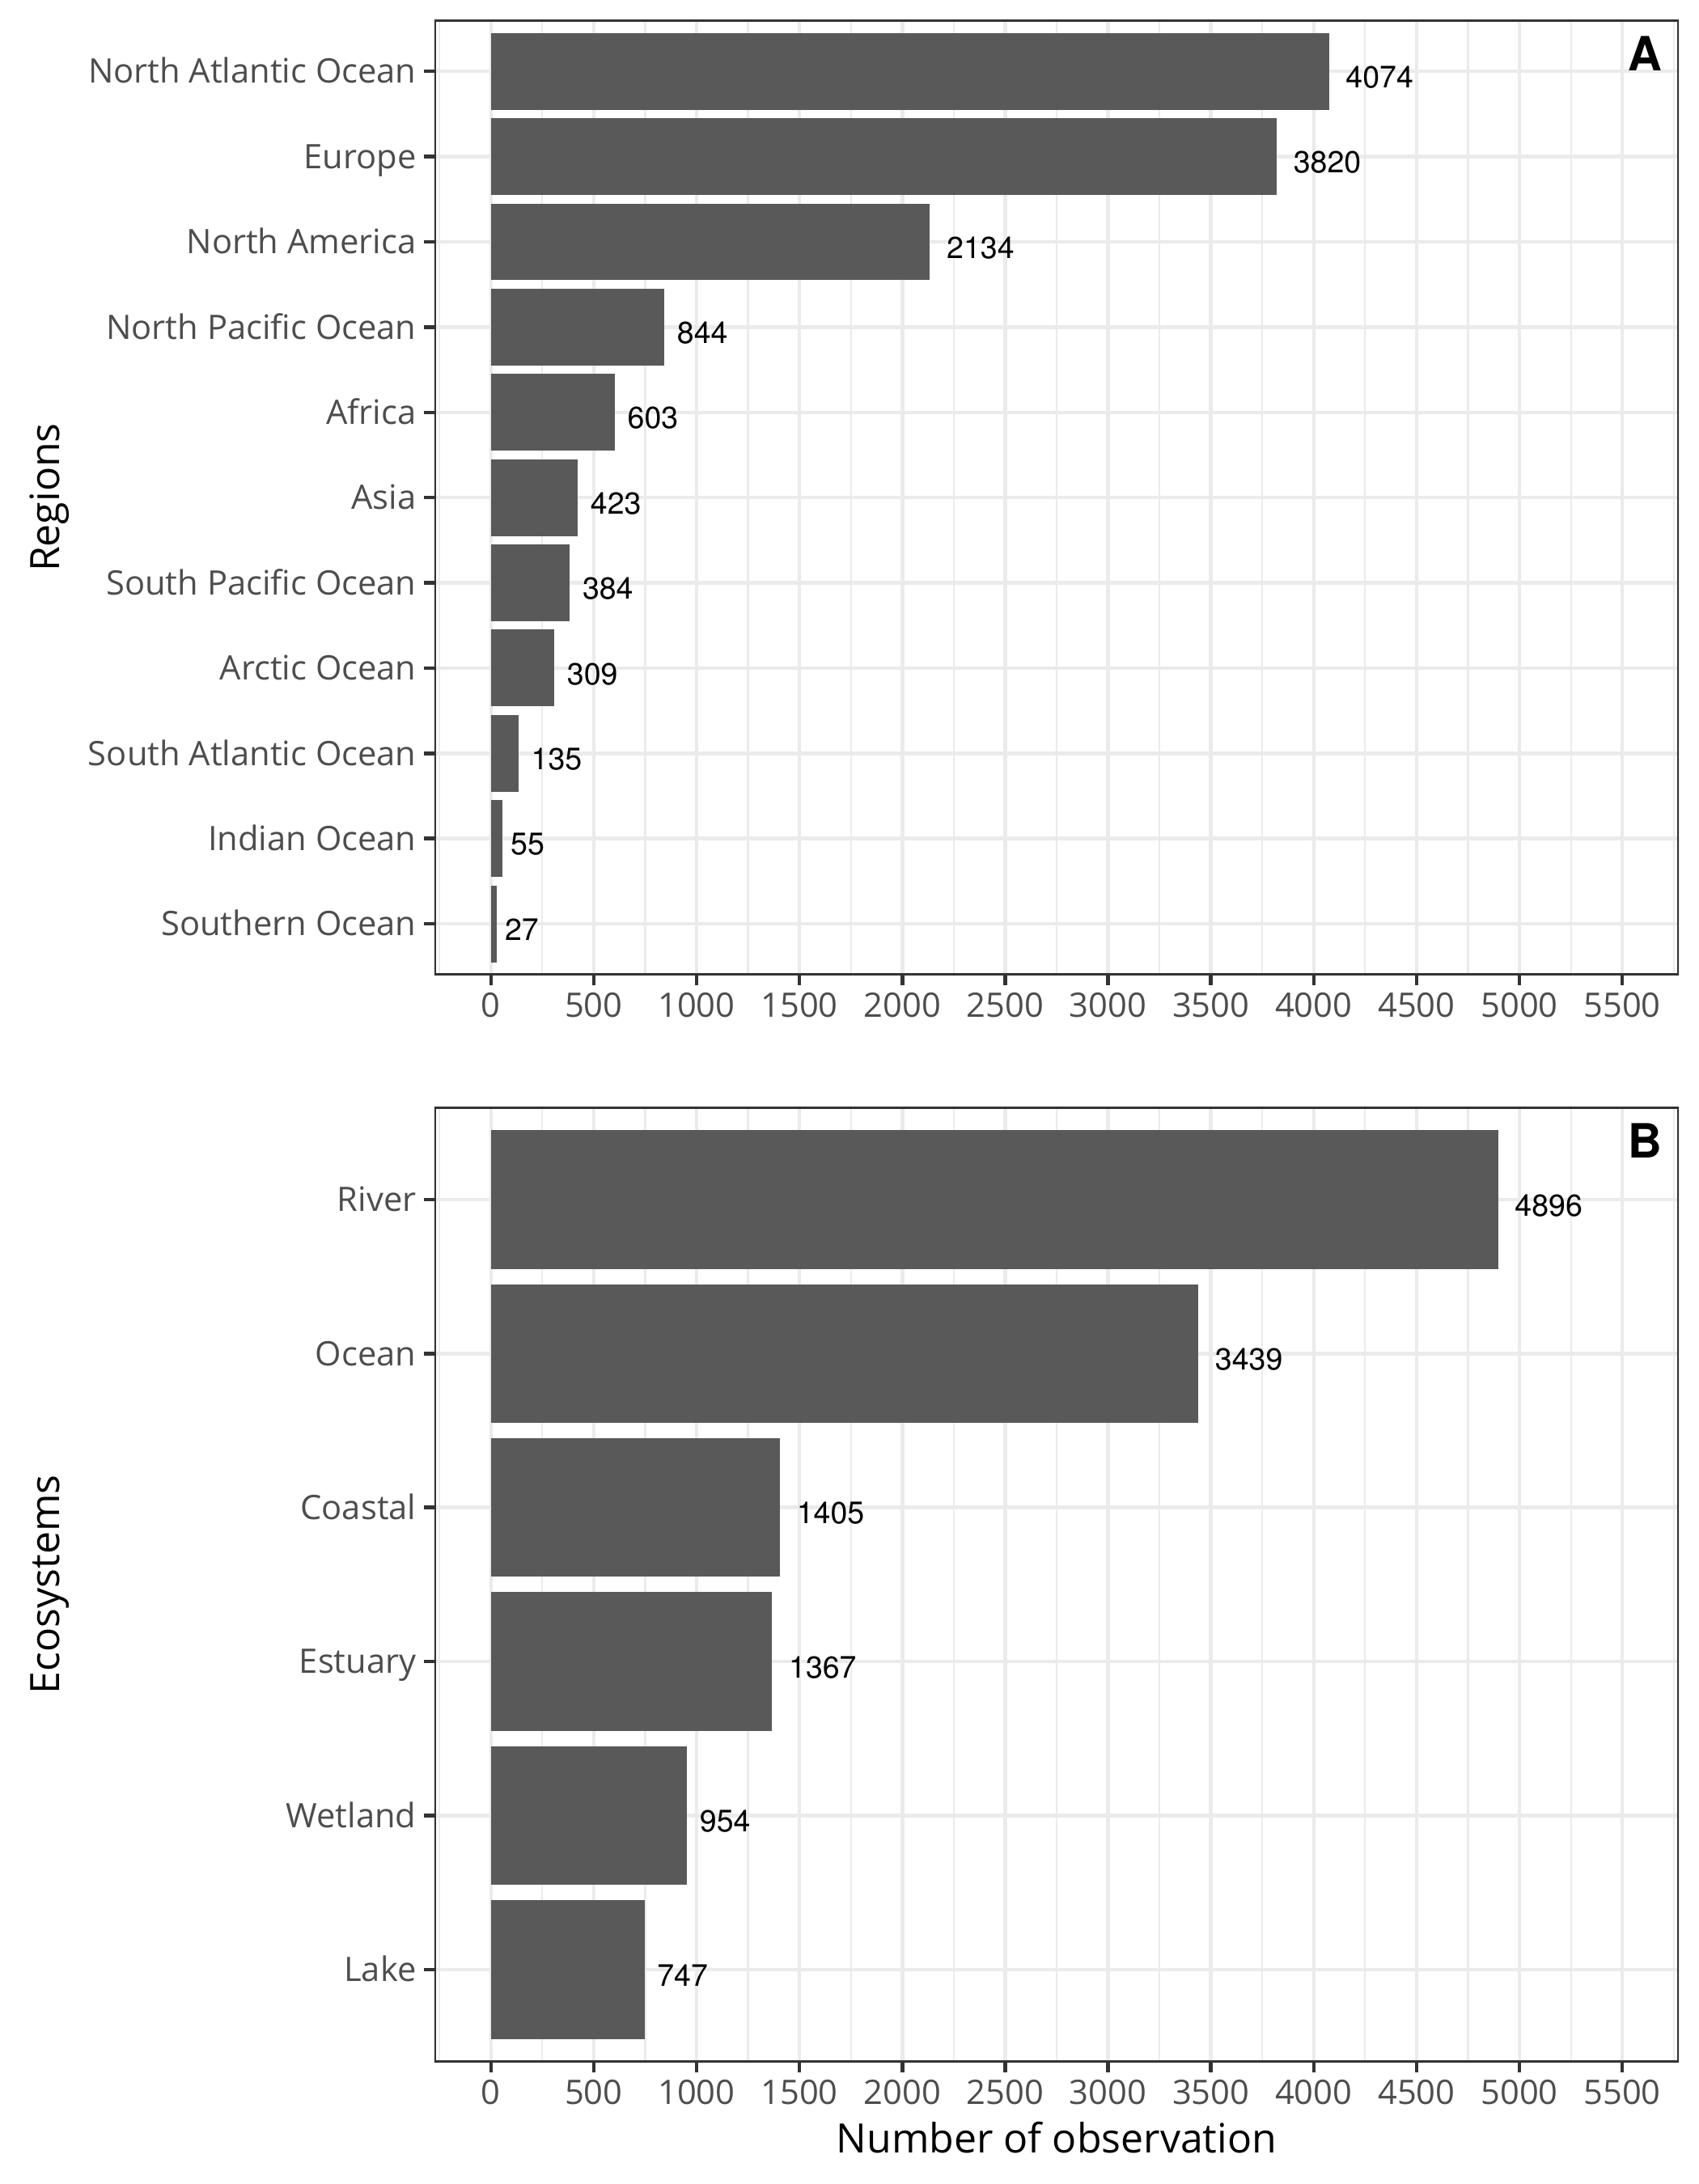
\includegraphics[scale = 0.85]{../../graphs/appendix1}
	\caption{Barplot showing the number of unique observations for (\textbf{A}) principal regions and (\textbf{B}) ecosystems.}
\end{figure}

\clearpage
\newpage

\section*{Supplementary section 2}
\subsection*{Estimation of \boldmath{$a_{\text{CDOM}}(350)$} from other wavelengths}

In the literature data, we found that a wide range of different wavelengths (between 250 and 490 nm) were used as reference wavelength to report absorption coefficients of CDOM (Supplementary Table 1). To make absorption coefficients comparable among studies, an interpolation procedure was used to estimate $a_{\text{CDOM}}(350)$ independently of the wavelength reported in each study. Between 250 and 350 nm, determination coefficients ($R^2$) gradually increased from 0.987 to 1 (Fig.~\ref{first}--A). After 350 nm, $R^2$ decreased rapidly to reach 0.86 at 500 nm. Between 250 and 500 nm, the regression slopes increased almost exponentially (0.28--6.99, Fig.~\ref{first}--B) whereas the intercepts increased more or less linearly between -1.4 and 1.5 m$^{-1}$ across the spectral range (Fig.~\ref{first}--C). Perfect fit at 350 nm is identified using vertical dashed lines where $R^2$ = 1, slope = 1 and intercept = 0. Note that the 95\% confidence interval of the estimated slope values is hardly distinguishable which emphasizes the robustness of the generated models (shaded area in Fig.~\ref{first}--B). Regression coefficients used to estimate $a_{\text{CDOM}}(350)$ in this study are presented in Supplementary Table 1. Absorption coefficients measured at wavelengths higher than 412 nm were not used to estimate absorption coefficients as 350 nm because of the $R^2$ below the selected threshold of 0.98. Supplementary Fig.~\ref{second} presents a heat map plot showing the $R^2$ of the regressions between all possible pairs of wavelengths between 250 nm and 500 nm (1 nm increment, $n$ = 63001). Corresponding coefficients are provided as a supplementary comma-separated values (CSV) file that enable the calculation of a given wavelength from another in the range of 250--500 nm.

% latex table generated in R 3.3.1 by xtable 1.8-2 package
% Mon Aug 29 14:20:13 2016
\begin{table}[ht]
\centering
\begin{tabular}{ccccr}
  \hline
Wavelength (nm) & Intercept & Slope & $R^2$ & $n$ \\ 
  \hline
253 & -1.27 & 0.28 & 0.9874 & 30 \\ 
  254 & -1.26 & 0.28 & 0.9876 & 5172 \\ 
  275 & -1.05 & 0.35 & 0.9907 & 76 \\ 
  280 & -0.98 & 0.37 & 0.9915 & 140 \\ 
  295 & -0.64 & 0.46 & 0.9947 & 76 \\ 
  300 & -0.54 & 0.49 & 0.9955 & 315 \\ 
  305 & -0.46 & 0.52 & 0.9962 & 98 \\ 
  320 & -0.26 & 0.64 & 0.9980 & 134 \\ 
  325 & -0.19 & 0.69 & 0.9987 & 412 \\ 
  330 & -0.14 & 0.74 & 0.9992 & 27 \\ 
  340 & -0.08 & 0.86 & 0.9997 & 29 \\ 
  355 & 0.02 & 1.08 & 0.9999 & 1183 \\ 
  365 & 0.11 & 1.27 & 0.9990 & 45 \\ 
  370 & 0.13 & 1.38 & 0.9984 & 595 \\ 
  375 & 0.14 & 1.50 & 0.9978 & 923 \\ 
  380 & 0.17 & 1.63 & 0.9968 & 899 \\ 
  400 & 0.28 & 2.25 & 0.9903 & 975 \\ 
  412 & 0.36 & 2.69 & 0.9841 & 1689 \\ 
  420 & 0.44 & 3.02 & 0.9786 & 59 \\ 
  440 & 0.64 & 3.95 & 0.9608 & 234 \\ 
  443 & 0.66 & 4.10 & 0.9566 & 1554 \\ 
  490 & 1.32 & 6.51 & 0.8807 & 606 \\ 
   \hline
\end{tabular}
\caption{Coefficients of the linear regressions between absorption 
coefficents at 350 nm and other wavelengths. Each regression includes a total 
of 2321 observations. All regression have p-value < 0.00001.  $n$ represents 
the number of observations used in this study that were reported at this 
wavelength.} 
\end{table}


\begin{figure}[h]
	\ContinuedFloat*
	\centering
	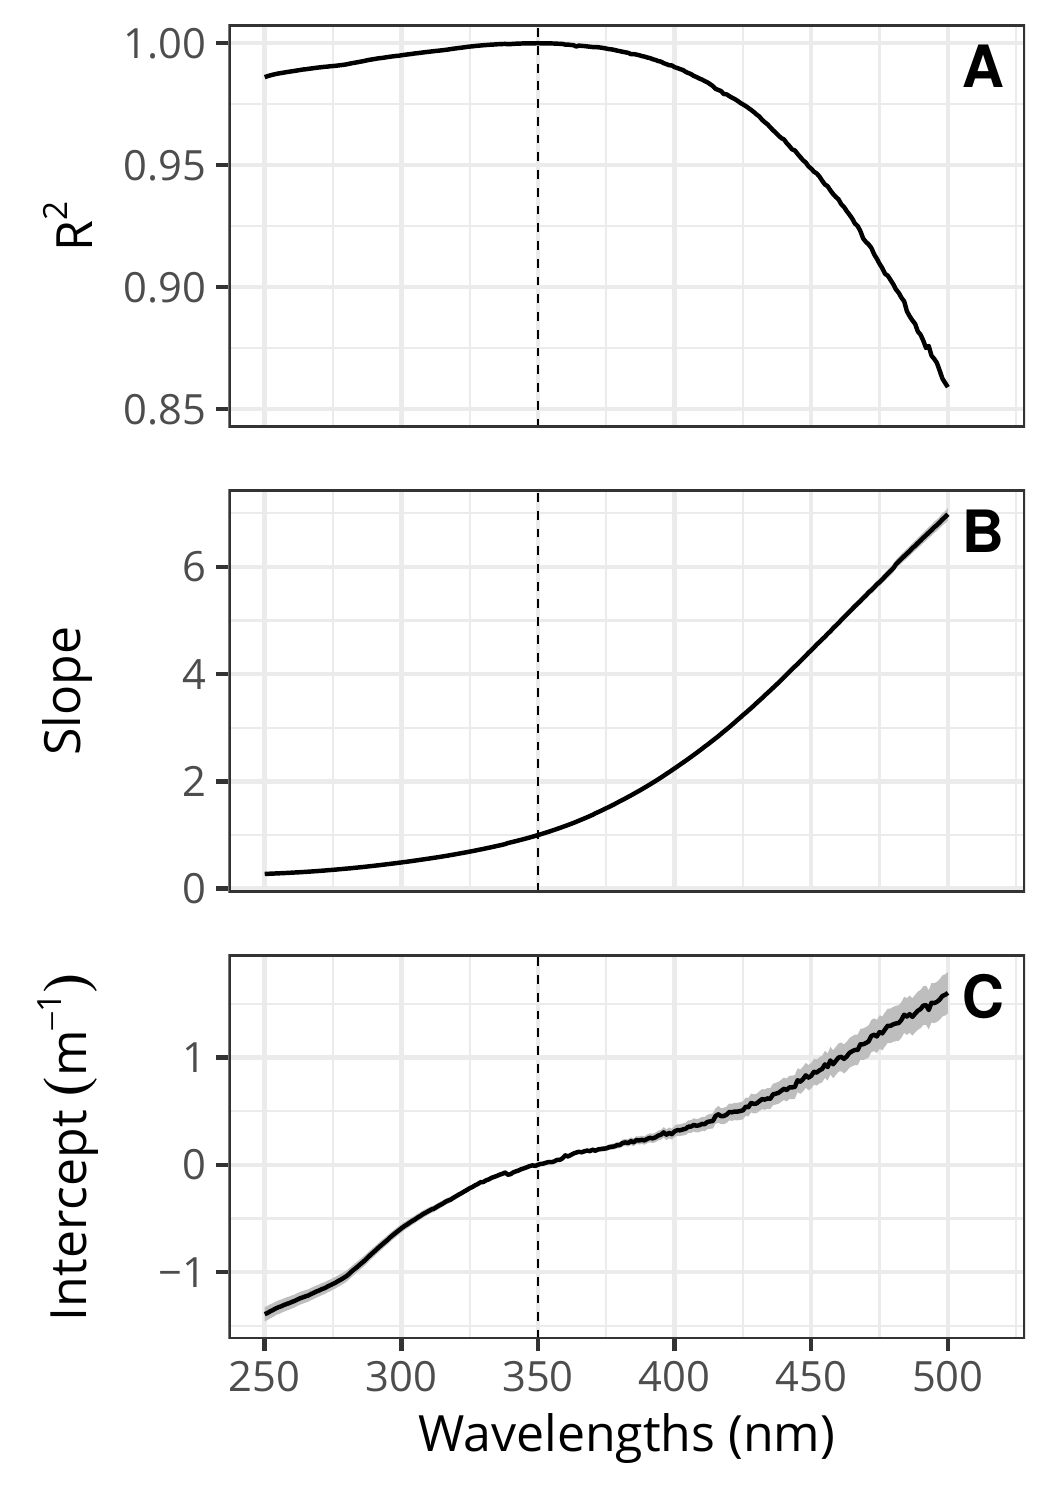
\includegraphics[scale = 1]{../../graphs/appendix2a}
	\caption{\label{first}Results of the linear regressions between a\textsubscript{CDOM}(350) and a\textsubscript{CDOM}($\lambda$). (\textbf{A}) Determination coefficients ($R^2$), (\textbf{B}) slopes and (\textbf{C}) intercepts of the linear regressions. Shaded areas (only visible in panel C) show the 95\% confidence interval of the estimated parameters. Panels contain the results of 251 linear models (one for each wavelength), each based on 2431 data points. Note that at $\lambda = 350$ nm (vertical dashed line), $R^2 = 1$, slope = 1 and intercept = 0. Note that for the Nelson et al. (2010) dataset (Table 1), absorption spectra were only available between 275 and 600 nm, and not included in this analysis.}
\end{figure}

\begin{figure}[h]
	\ContinuedFloat
	\centering
	\includegraphics[scale = 1]{../../graphs/appendix2b}
	\caption{\label{second}Heat map showing the determination coefficients ($R^2$) of the linear regressions between absorption values for each pair of wavelengths between 250 and 500 nm ($n = 63001, 0.83 \le R^2 \le 1$). Each regression is based on 2431 observations. Note that the diagonal of the plot shows $R^2 = 1$. }
\end{figure}

\clearpage
\newpage

\section*{Supplementary section 3}
\subsection*{Log-linear relationship between \boldmath{$a_{\text{CDOM}}(350)$} and DOC divided by ecosystems.}

\begin{figure}[h]
	\centering
	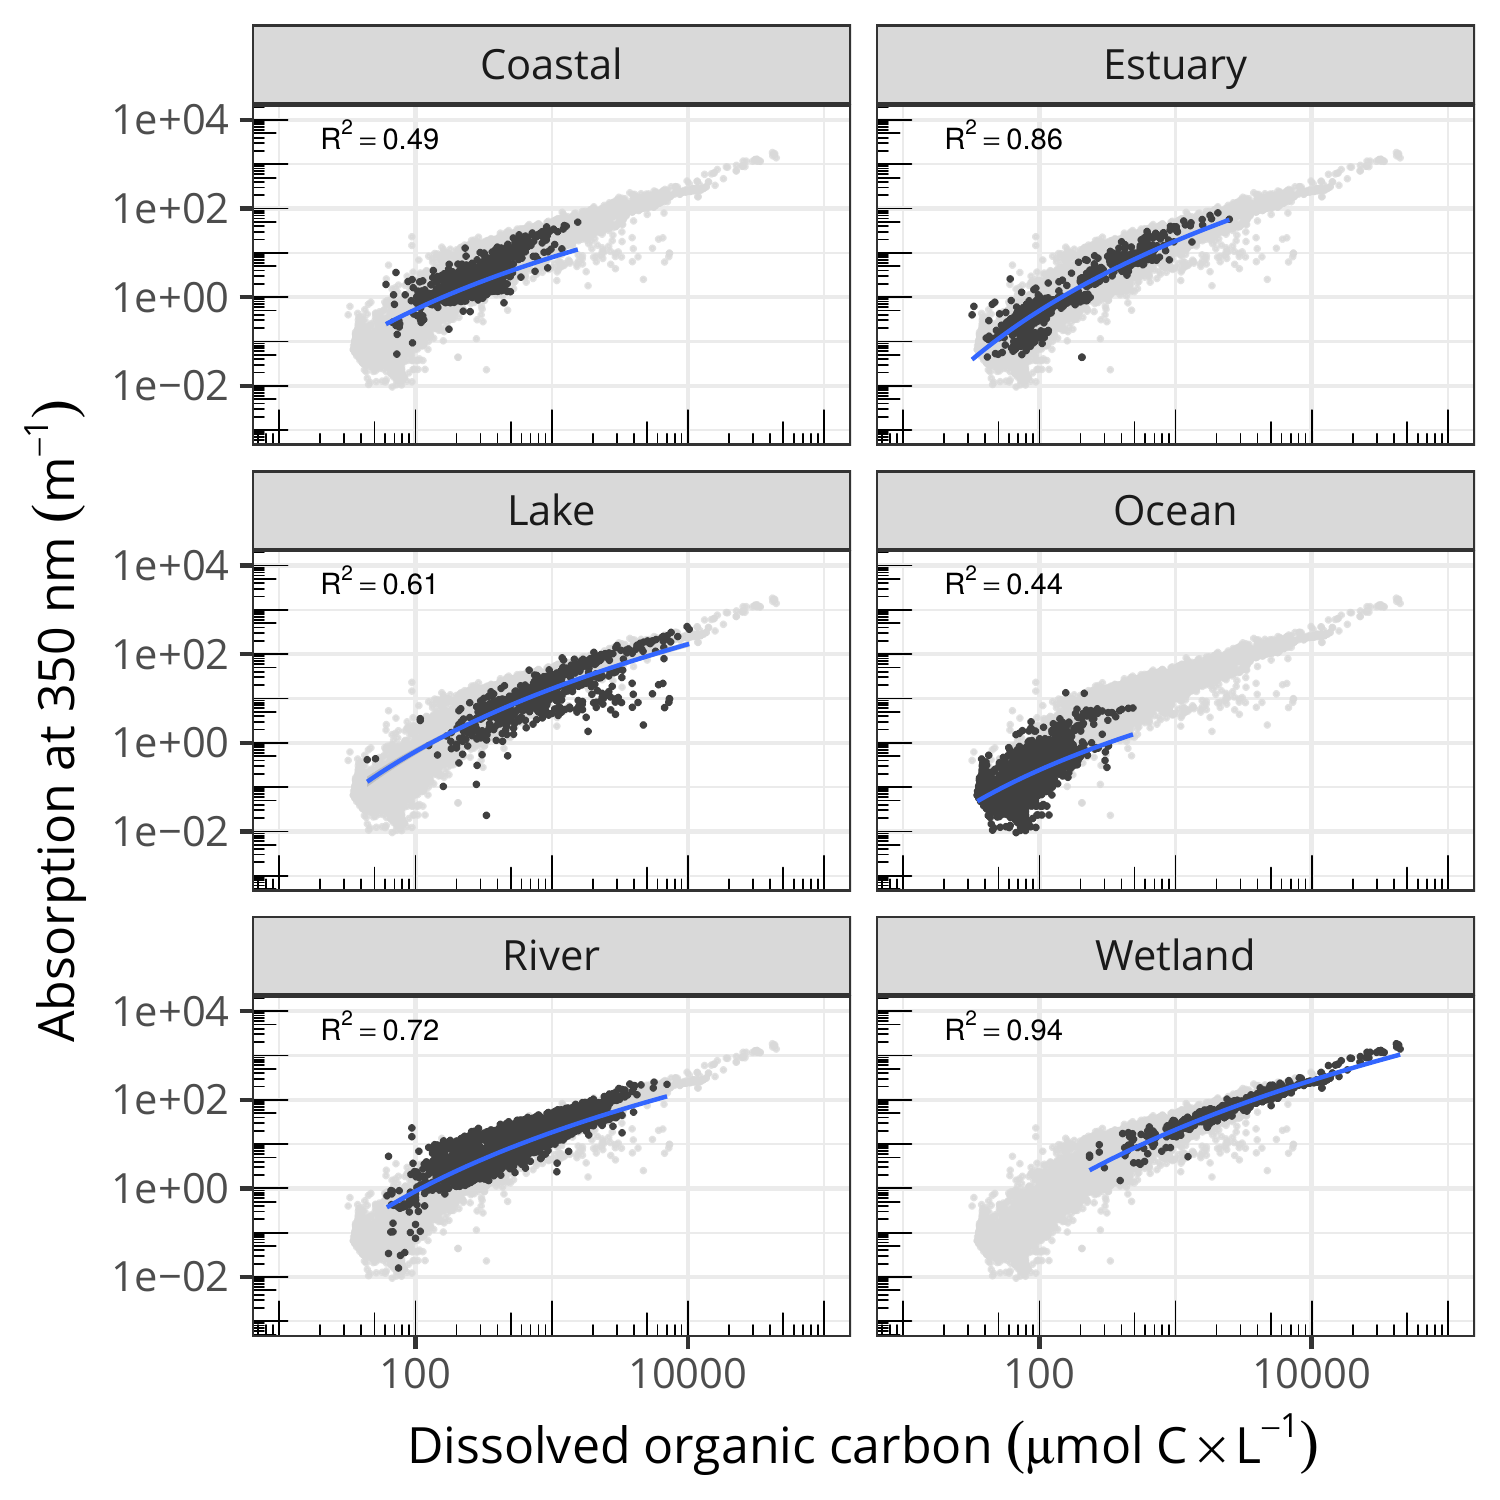
\includegraphics[scale = 1]{../../graphs/appendix3}
	\caption{The blue line is the fitted values of a linear model $y = \log(x)$. The shaded areas represent the 95\% confidence intervals. A total of 12808 observations are distributed across all panels (light gray dots in the background show the same global relation presented in Fig. 4).}
\end{figure}

\clearpage
\newpage

\section*{Supplementary section 4}
\subsection*{Residuals analysis}

\begin{figure}[H]
	\centering
	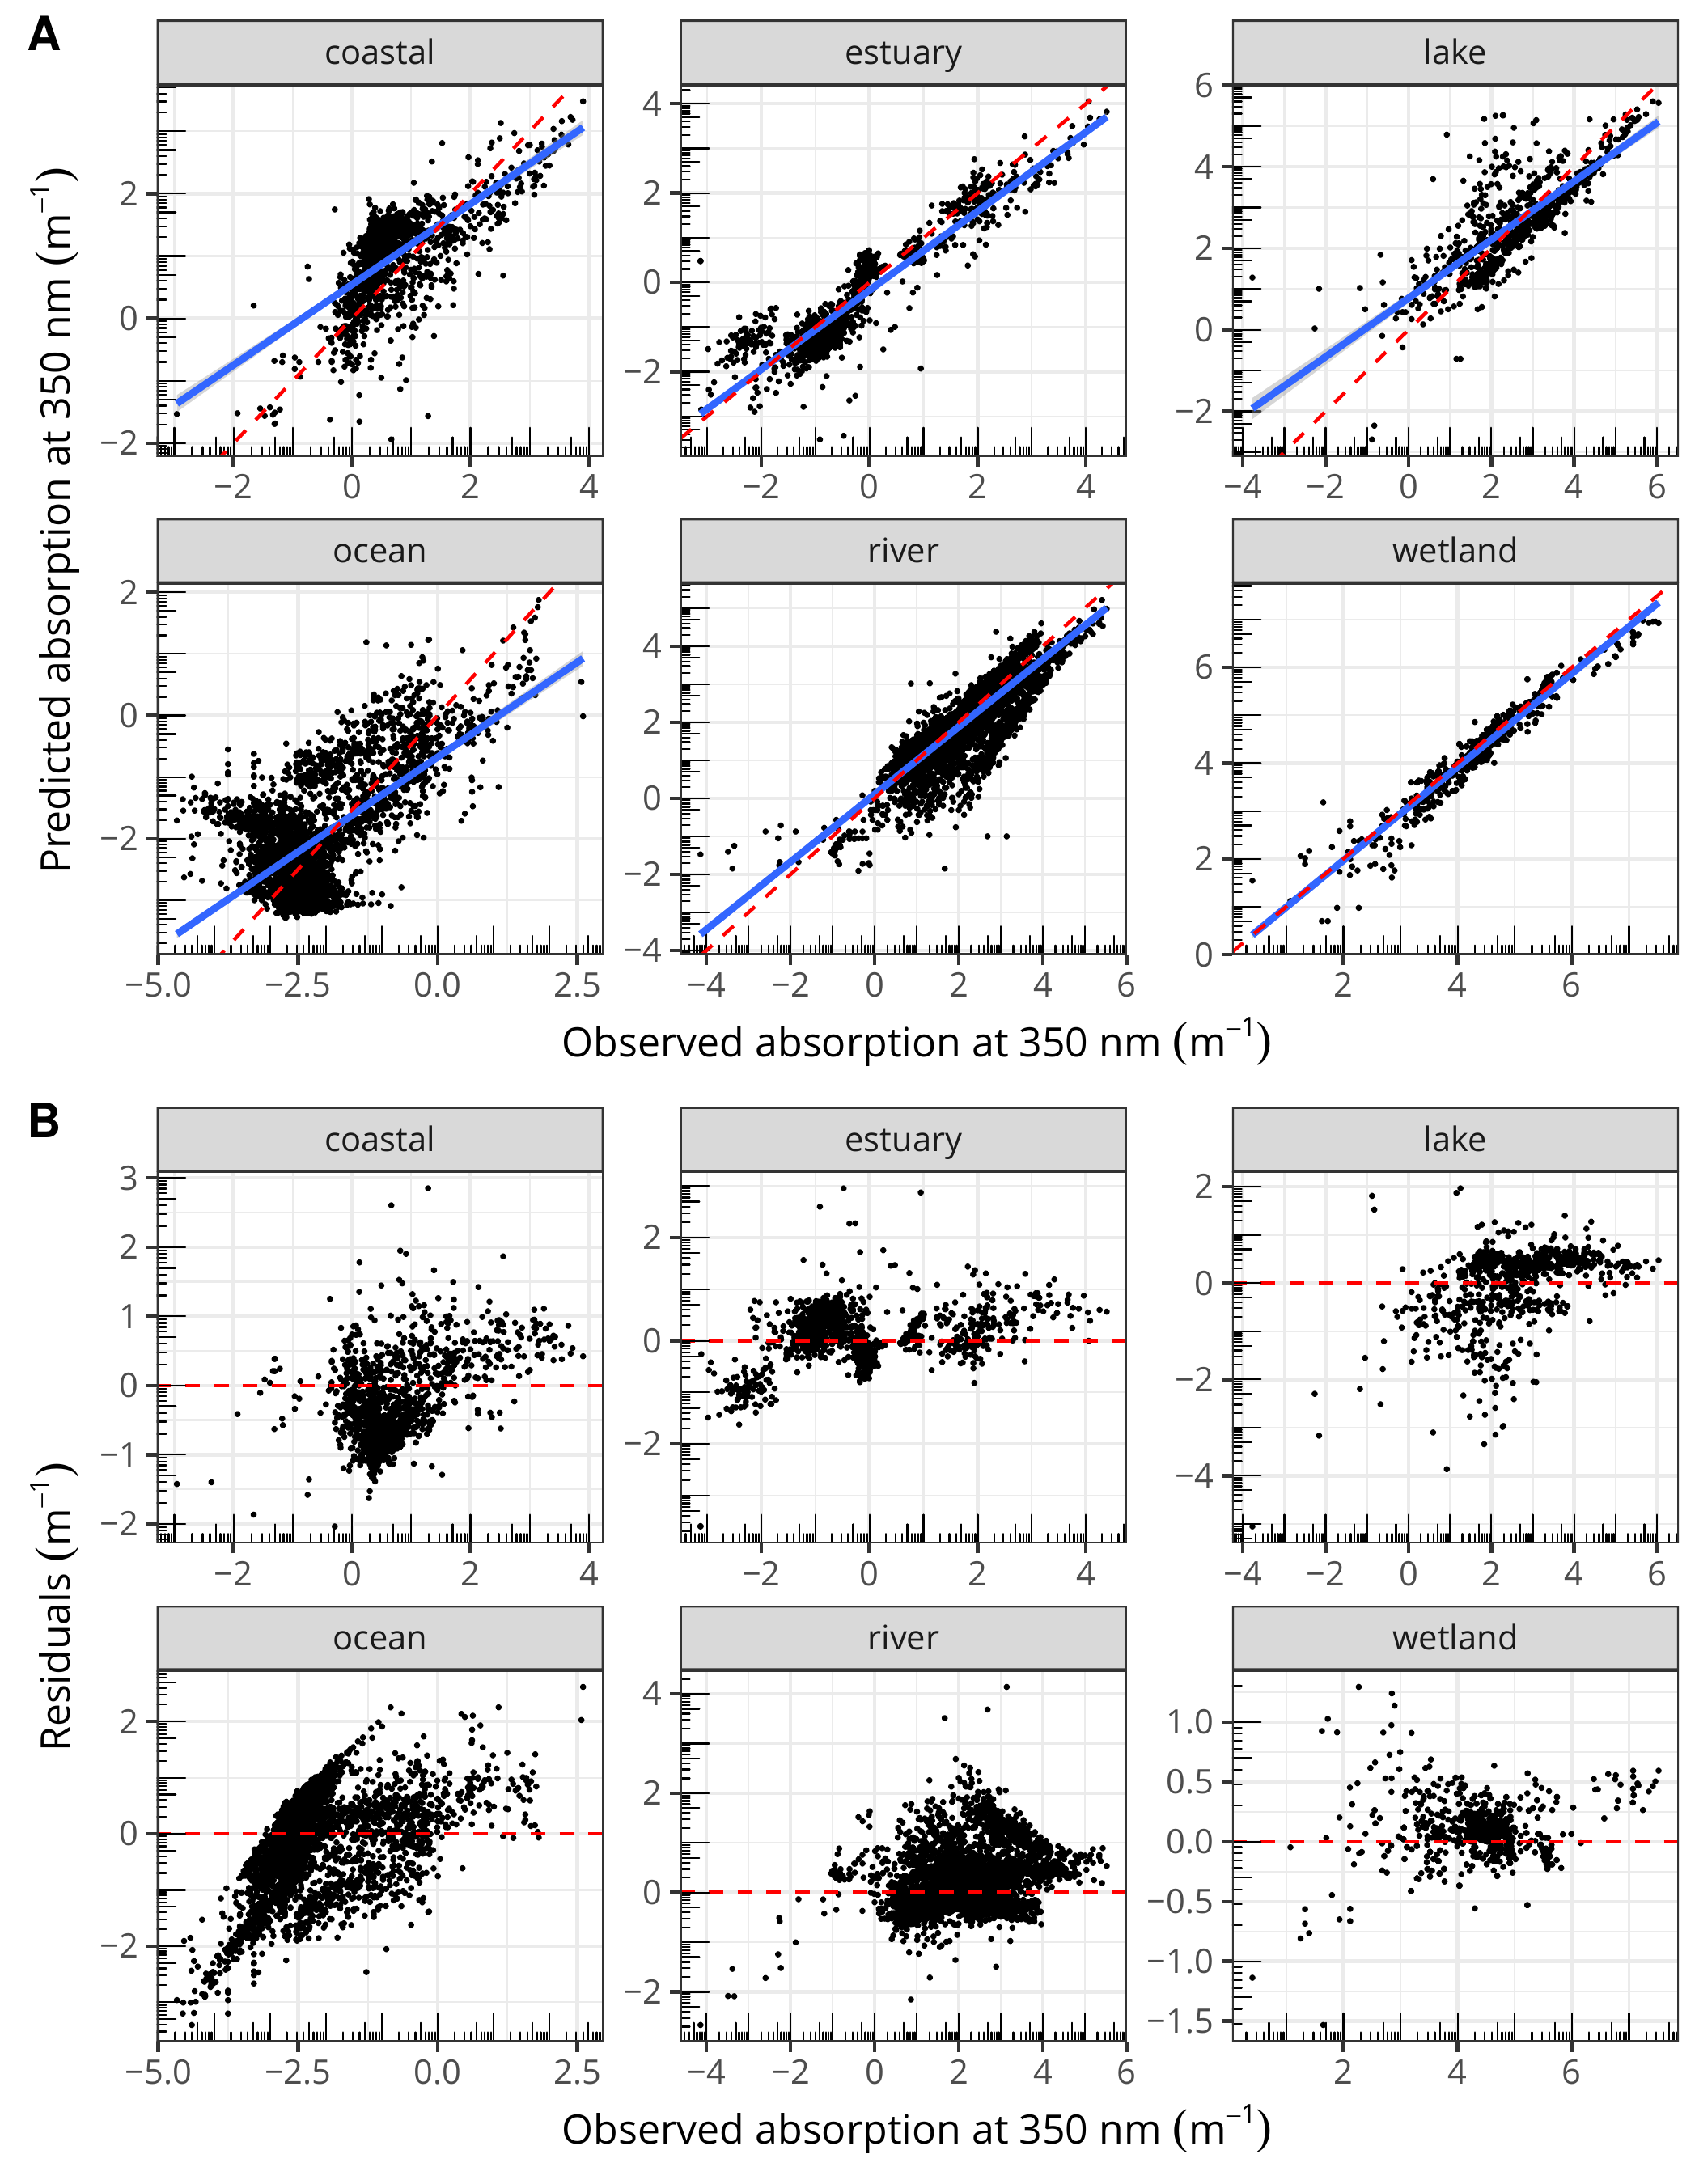
\includegraphics[scale = 0.8]{../../graphs/appendix4}
	\caption{\textbf{A} Scatterplots showing the relationship between observed and predicted values of $a_{\text{CDOM}}(350)$ (see Fig. 4). \textbf{B} Associated residual plots.}
\end{figure}

\clearpage
\newpage

\section*{Supplementary section 5}
\subsection*{Temporal and spatial distribution of the data}

\begin{figure}[h]
	\centering
	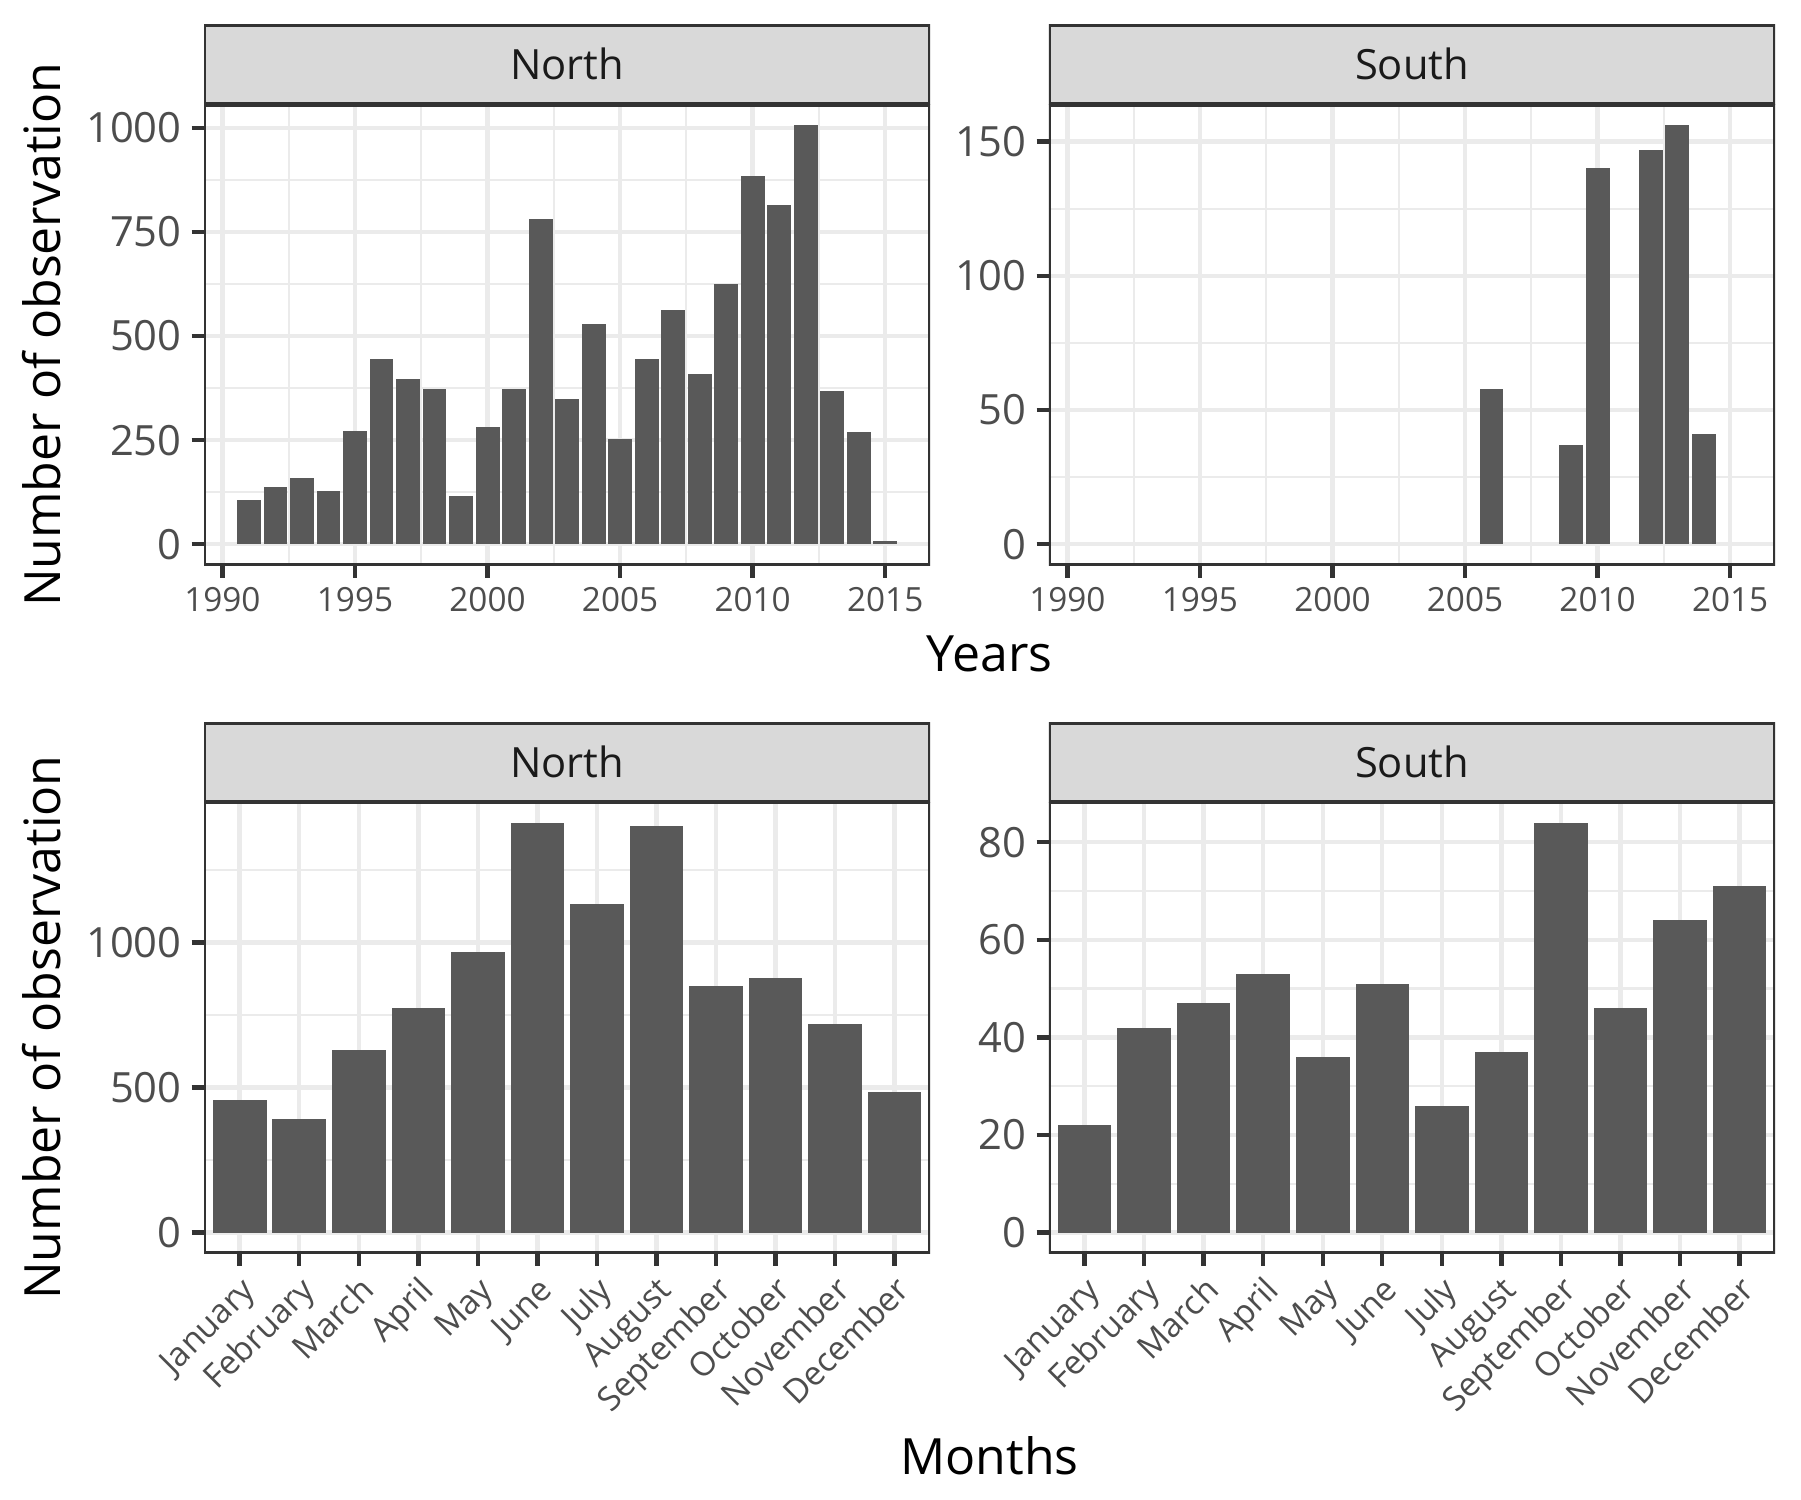
\includegraphics[scale = 1]{../../graphs/appendix5}
	\caption{Barplots showing how the data is distributed temporally across North and South hemisphere ($n = 12808$).}
\end{figure}

\clearpage
\newpage

\section*{Supplementary section 6}
\subsection*{Results of the Tukey Honest Significant Differences}

The following tables present the results of Anova's and their associated post-hoc the Tukey Honest Significant Differences for each variables presented in Fig. 3.

\subsubsection*{CDOM absorption}

% latex table generated in R 3.4.0 by xtable 1.8-2 package
% Mon Jun 19 10:06:17 2017
\begin{table}[ht]
\centering
\begin{tabular}{rrrrr}
  \hline
Df & Sum Sq & Mean Sq & F value & Pr(>F) \\ 
  \hline
5 & 12811085.15 & 2562217.03 & 851.56 & 0.0000 \\ 
  12802 & 38519112.74 & 3008.84 &  &  \\ 
   \hline
\end{tabular}
\caption{Anova results of $a_{\text{CDOM}}(350)$ among ecosystems (See Fig. 3A).} 
\end{table}

% latex table generated in R 3.4.0 by xtable 1.8-2 package
% Mon Jun 19 09:52:47 2017
\begin{table}[ht]
\centering
\begin{tabular}{lrrrr}
  \hline
comparison & estimate & conf.low & conf.high & adj.p.value \\ 
  \hline
Lake-Wetland & -97.80 & -105.43 & -90.16 & 0.00 \\ 
  River-Wetland & -109.53 & -115.06 & -104.00 & 0.00 \\ 
  Coastal-Wetland & -122.29 & -128.84 & -115.73 & 0.00 \\ 
  Estuary-Wetland & -122.89 & -129.48 & -116.29 & 0.00 \\ 
  Ocean-Wetland & -125.10 & -130.82 & -119.38 & 0.00 \\ 
  River-Lake & -11.73 & -17.87 & -5.59 & 0.00 \\ 
  Coastal-Lake & -24.49 & -31.57 & -17.41 & 0.00 \\ 
  Estuary-Lake & -25.09 & -32.21 & -17.98 & 0.00 \\ 
  Ocean-Lake & -27.31 & -33.62 & -21.00 & 0.00 \\ 
  Coastal-River & -12.76 & -17.49 & -8.03 & 0.00 \\ 
  Estuary-River & -13.36 & -18.14 & -8.58 & 0.00 \\ 
  Ocean-River & -15.57 & -19.05 & -12.10 & 0.00 \\ 
  Estuary-Coastal & -0.60 & -6.54 & 5.34 & 1.00 \\ 
  Ocean-Coastal & -2.82 & -7.77 & 2.13 & 0.58 \\ 
  Ocean-Estuary & -2.21 & -7.21 & 2.79 & 0.81 \\ 
   \hline
\end{tabular}
\caption{Tukey Honest Significant Differences between the means of $a_{\text{CDOM}}(350)$ among ecosystems (See Fig. 3A).} 
\end{table}


\clearpage
\newpage

\subsubsection*{Dissolved organic carbon}
% latex table generated in R 3.4.0 by xtable 1.8-2 package
% Mon Jun 19 09:52:47 2017
\begin{table}[ht]
\centering
\begin{tabular}{rrrrr}
  \hline
Df & Sum Sq & Mean Sq & F value & Pr(>F) \\ 
  \hline
5 & 15374521101.54 & 3074904220.31 & 1388.90 & 0.0000 \\ 
  12802 & 28342521862.43 & 2213913.60 &  &  \\ 
   \hline
\end{tabular}
\caption{Anova results of DOC among ecosystems (See Fig. 3A).} 
\end{table}

% latex table generated in R 3.4.0 by xtable 1.8-2 package
% Mon Jun 19 09:52:47 2017
\begin{table}[ht]
\centering
\begin{tabular}{lrrrr}
  \hline
comparison & estimate & conf.low & conf.high & adj.p.value \\ 
  \hline
Lake-Wetland & -3182.94 & -3390.13 & -2975.76 & 0.00 \\ 
  River-Wetland & -3656.27 & -3806.35 & -3506.19 & 0.00 \\ 
  Coastal-Wetland & -4113.91 & -4291.81 & -3936.00 & 0.00 \\ 
  Estuary-Wetland & -4241.80 & -4420.70 & -4062.89 & 0.00 \\ 
  Ocean-Wetland & -4357.47 & -4512.65 & -4202.29 & 0.00 \\ 
  River-Lake & -473.33 & -639.91 & -306.75 & 0.00 \\ 
  Coastal-Lake & -930.96 & -1122.99 & -738.93 & 0.00 \\ 
  Estuary-Lake & -1058.85 & -1251.81 & -865.90 & 0.00 \\ 
  Ocean-Lake & -1174.53 & -1345.71 & -1003.34 & 0.00 \\ 
  Coastal-River & -457.63 & -585.98 & -329.29 & 0.00 \\ 
  Estuary-River & -585.53 & -715.25 & -455.80 & 0.00 \\ 
  Ocean-River & -701.20 & -795.55 & -606.85 & 0.00 \\ 
  Estuary-Coastal & -127.89 & -289.00 & 33.22 & 0.21 \\ 
  Ocean-Coastal & -243.57 & -377.84 & -109.29 & 0.00 \\ 
  Ocean-Estuary & -115.67 & -251.27 & 19.92 & 0.15 \\ 
   \hline
\end{tabular}
\caption{Tukey Honest Significant Differences between the means of DOC among ecosystems (See Fig. 3B).} 
\end{table}


\clearpage
\newpage

\subsubsection*{Specific UV absorbance}
% latex table generated in R 3.4.0 by xtable 1.8-2 package
% Mon Jun 19 10:06:17 2017
\begin{table}[ht]
\centering
\begin{tabular}{rrrrr}
  \hline
Df & Sum Sq & Mean Sq & F value & Pr(>F) \\ 
  \hline
5 & 2193.88 & 438.78 & 1981.10 & 0.0000 \\ 
  12802 & 2835.40 & 0.22 &  &  \\ 
   \hline
\end{tabular}
\caption{Anova results of $\text{SUVA}_{350}$ among ecosystems (See Fig. 3A).} 
\end{table}

% latex table generated in R 3.4.0 by xtable 1.8-2 package
% Mon Jun 19 10:06:17 2017
\begin{table}[ht]
\centering
\begin{tabular}{lrrrr}
  \hline
comparison & estimate & conf.low & conf.high & adj.p.value \\ 
  \hline
Lake-Wetland & -0.34 & -0.41 & -0.28 & 0.00 \\ 
  River-Wetland & -0.36 & -0.40 & -0.31 & 0.00 \\ 
  Estuary-Wetland & -0.95 & -1.01 & -0.90 & 0.00 \\ 
  Coastal-Wetland & -0.90 & -0.96 & -0.85 & 0.00 \\ 
  Ocean-Wetland & -1.21 & -1.26 & -1.17 & 0.00 \\ 
  River-Lake & -0.01 & -0.06 & 0.04 & 0.99 \\ 
  Estuary-Lake & -0.61 & -0.67 & -0.55 & 0.00 \\ 
  Coastal-Lake & -0.56 & -0.62 & -0.50 & 0.00 \\ 
  Ocean-Lake & -0.87 & -0.92 & -0.82 & 0.00 \\ 
  Estuary-River & -0.60 & -0.64 & -0.56 & 0.00 \\ 
  Coastal-River & -0.55 & -0.59 & -0.51 & 0.00 \\ 
  Ocean-River & -0.86 & -0.89 & -0.83 & 0.00 \\ 
  Coastal-Estuary & 0.05 & -0.00 & 0.10 & 0.06 \\ 
  Ocean-Estuary & -0.26 & -0.30 & -0.22 & 0.00 \\ 
  Ocean-Coastal & -0.31 & -0.35 & -0.27 & 0.00 \\ 
   \hline
\end{tabular}
\caption{Tukey Honest Significant Differences between the means of $\text{SUVA}_{350}$ among ecosystems (See Fig. 3C).} 
\end{table}


\clearpage
\newpage

\section*{Supplementary section 7}
\subsection*{Effect of salinity and sampling depth on the relationship between DOC and CDOM absorption}

In this section we explore what are the consequences of changing the arbitrary salinity threshold used in the paper from 30 to 32. In the Supplementary Fig. \ref{fig:salinity} one can see a good positive relationship for samples with salinity $\le$ 32 (right panel). One can also see the negative relationship documented by Nelson \& Siegel (2013) which is represented by the blue points in the left panel. One characteristic of the these sample points is that they are associated with low DOC content (< 100 µmol C). One possible explanation behind this negative relationship is that at low DOC, carbon content and color are likely to be decoupled. We can also observe that at salinity > 32, a good relationship between DOC and $a_{\text{CDOM}}(350)$ is possible (red points in left panel), suggesting that salinity might not be a good proxy for estimating the ``strength'' of the relation. We believe that influence of terrestrial inputs (estimated by the distance to the closest shoreline) is a better proxy for assessing the quality of the between DOC and $a_{\text{CDOM}}(350)$ relationship (see Fig. 5 in the main text).

\begin{figure}[H]
	\centering
	\includegraphics[scale = 0.7]{../../graphs/appendix7}
	\caption{Effect of salinity and sampling depth on the relationship between DOC and CDOM absorption.}
	\label{fig:salinity}
\end{figure}

Finally, we explored the data to find out if the sampling depth could induce bias or patterns in the observed relationship. In the paper we precise that 81\% of oceanic samples were located at depth < 1800 m  which is the threshold often used to classify observations as ``deep sea''. Because we do not have the information of the mixing layer available for each study, we arbitrarily chosen a value of 500~m to make the distinction between surface and deep samples. As one can see in the previous figure, both surface (< 500 m) and deep observations ($\ge$ 500 m) are overlapping homogeneously suggesting that sampling depth is not likely to induce bias (at least at global scale). This can be viewed on the left panel where the regression lines for shallow and deep open marine water (salinity > 32) aligns almost perfectly.

\end{document}
